%%%%%%%%%%%%%%%%%%%%%%%%%%%%%%%%%%%%%%%%%%%%%%%%%%%%%%%%%%%%%%%%%%%%%%%%%%
%% Review Volume (last updated on 2014/03/05) %%
%% Trim Size: 9.61in x 6.69in %%
%% Text Area: 8in (include runningheads) x 5in %%
%% Main Text: 10 on 13pt %%
%% For support: Yolande Koh, <ykoh@wspc.com.sg> %%
%% D. Rajesh Babu, <rajesh@wspc.com.sg> %%
%%%%%%%%%%%%%%%%%%%%%%%%%%%%%%%%%%%%%%%%%%%%%%%%%%%%%%%%%%%%%%%%%%%%%%%%%%
%%
%\documentclass[wsdraft]{ws-rv961x669} % to draw border line around text area
%\documentclass{ws-rv961x669}
\documentclass[addchapnum]{ws-rv961x669} % to add chapter number in volume
\usepackage{ws-rv-van} % numbered citation/references (default)
%\usepackage{ws-rv-thm} % comment this line when `amsthm / theorem / ntheorem` package is used
%\usepackage{subfigure} % required only when side-by-side / subfigures are used
\usepackage{ws-index} % required only when multiple indexes are used
%\usepackage[colorlinks=false]{hyperref}
%\usepackage{doi}
\usepackage{bbm}
\usepackage{amsmath}
\usepackage{amssymb}
\makeindex
\newindex{aindx}{adx}{and}{Author Index} % author index
\renewindex{default}{idx}{ind}{Subject Index} % subject index

\newcommand{\req}[1]{Eq.~(\ref{#1})}
 
\begin{document}

\chapter[Dynamics flavor mixing through transition moments]{Dynamics flavor mixing through transition moments\label{JR_ch1}}

\author[J. Rafelski and A. Steinmetz]{Johann Rafelski and Andrew Steinmetz\footnote{JohannR@Arizona.EDU,AJSteinmetz@Arizona.EDU}}
\aindx{Rafelski, J.}
\aindx{Steinmetz, A.}

\address{Department of Physics, The University of Arizona, Tucson, AZ 85721, USA}

\begin{abstract} 
As neutrinos are naturally massless in the standard model the observed flavor oscillation presents a problem. Moreover it is unknown if neutrinos are Dirac-type or Majorana-type fermions. We show that the required neutrino flavor mixing can be driven by electromagnetic transition dipole moment. We analyze sensitivity of the rotation mixing matrix to strong electromagnetic fields.
\end{abstract}

\markboth{Johann Rafelski and Andrew Steinmetz}{Neutrinos in EM fields} % Customized running heads

\body

%\tableofcontents\

%%%%%%%%%%%%%%%%%%%%%%%%%%%%%%%%%%%%
\section{Introduction}
\label{sec:intro}
%%%%%%%%%%%%%%%%%%%%%%%%%%%%%%%%%%%%

In this work we look at the connection between neutrino transition magnetic dipole moments~\cite{Shrock:1980vy,Shrock:1982sc} and neutrino flavor oscillation. Neutrinos once were the dominant form of energy density in the universe~\cite{Rafelski:2023emw} and are also important in the context of stellar evolution and supernova. There is profound interest in understanding their physical properties due to their importance as a bridge to beyond standard model (BSM) physics~\cite{DUNE:2020fgq}. It is also unknown which hierarchy neutrinos follow therefore probing the EM properties of neutrinos could contribute evidence for one model over the other. Their electromagnetic (EM) properties have been considered before~\cite{Giunti:2014ixa} but to best of our knowledge this is a first consideration of EM contribution to flavor oscillation.

The size of the neutrino magnetic dipole moment is relatively small with a lower bound determined by the standard model and an upper bound from reactor or solar observations given by~\citep{Studenikin:2016ykv,Canas:2015yoa,AristizabalSierra:2021fuc}
\begin{align}
    \label{momentbound:1}
    10^{-19}\mu_{B}<\mu_{\nu}^\mathrm{eff}<10^{-10}\mu_{B}\,,\qquad\mu_{B}=\frac{e\hbar}{2m}
\end{align}
where $\mu_{B}$ is the Bohr magneton and $\mu_{\nu}^\mathrm{eff}$ is the effective and characteristic size of the neutrino magnetic moment.

Considering higher order diagrams neutrino should manifestation non-minimal EM interactions~\citep{Shrock:1980vy} of the form
\begin{gather}
    \label{mu:1}
    \mu_{\ell\ell'}=
	\begin{pmatrix}
		\mu_{ee} & \mu_{e\mu} & \mu_{e\tau} \\
		\mu_{e\mu}^{*} & \mu_{\mu\mu} & \mu_{\mu\tau} \\
		\mu_{e\tau}^{*} & \mu_{\mu\tau}^{*} & \mu_{\tau\tau}
	\end{pmatrix}\,,
\end{gather}
where $\ell$ are the neutral lepton flavor indices $\ell\in\nu_{e},\nu_{\mu},\nu_{\tau}$. The transition moments are small~\cite{Shrock:1980vy} but BSM physics is capable of producing an abnormally large electromagnetic dipole~\citep{Lindner:2017uvt,Brdar:2020quo} within the bounds of~\req{momentbound:1} which may manifest itself in strong field or/and dense matter environments.

%%%%%%%%%%%%%%%%%%%%%%%%%%%%%%%%%%%%%%%
\section{Description of neutrino flavor mixing}
\label{sec:numass}
%%%%%%%%%%%%%%%%%%%%%%%%%%%%%
For clarity of presentation we recall briefly textbook level neutrino physics: Experiment shows that neutrino mass and flavor eigenstates differ. This misalignment between the two representations is described as rotation of the neutrino flavor 3-vector where $N=3$ is the number of generations. The unitary mixing matrix $V$ allows for the change of basis between mass and flavor eigenstates as 
\begin{alignat}{1}
	\label{basis:1} \nu_{\ell}=\sum_{k=1}^{3}V_{\ell k}\nu_{k}\,\rightarrow
	\begin{pmatrix}
		\nu_{e}\\
		\nu_{\mu}\\
		\nu_{\tau}
	\end{pmatrix}=
	\begin{pmatrix}
		V_{e1} & V_{e2} & V_{e3}\\
		V_{\mu1} & V_{\mu2} & V_{\mu3}\\
		V_{\tau1} & V_{\tau2} & V_{\tau3}
	\end{pmatrix}
	\begin{pmatrix}
		\nu_{1}\\
		\nu_{2}\\
		\nu_{3}
	\end{pmatrix}\,,
\end{alignat}
where $\nu_{\ell}$ is the neutrino state vector written in the flavor basis while in the mass basis we use $\nu_{k}$ with $k\in1,2,3$. Hereafter we will use implied summation  over repeated indices.

The parameterization of the components of the mixing matrix depends on the Dirac- or Majorana-nature of the neutrinos. We consider $U$ to be the Dirac neutrino matrix which in the standard parameterization~\citep{Schwartz:2014sze}, can be expressed as
\begin{alignat}{1}
	\label{rotation:1} U_{\ell k} =
	  \begin{pmatrix}
		  c_{12}c_{13} & s_{12}c_{13} & s_{13}e^{-i\delta}\\
		  -s_{12}c_{23} - c_{12}s_{13}s_{23}e^{i\delta} & c_{12}c_{23} - s_{12}s_{13}s_{23}e^{i\delta} & c_{13}s_{23}\\
		  s_{12}s_{23} - c_{12}s_{13}c_{23}e^{i\delta}& -c_{12}s_{23} - s_{12}s_{13}c_{23}e^{i\delta} & c_{13}c_{23}
	  \end{pmatrix}\,,
\end{alignat}
where $c_{ij} = \mathrm{cos}(\theta_{ij})$ and $s_{ij} = \mathrm{sin}(\theta_{ij})$. In this convention, the three mixing angles $(\theta_{12}, \theta_{13}, \theta_{23})$, are understood to be the Euler angles for generalized rotations and $\delta$ is the CP-violating complex phase. 

For the Majorana case of interest to us we must allow a greater number of complex phases described by an additional matrix $P$
\begin{alignat}{1}
	\label{phases:1} &V_{\ell k} = U_{\ell k'}P_{k'k}\,,\\
	\label{phases:3} &P_{kk'} = \mathrm{diag}(e^{i\rho},e^{i\sigma},1)\,.
\end{alignat}
Majorana neutrinos allow up to two additional complex phases $\rho$ and $\sigma$ which along with $\delta$ participate in CP-violation. The mixing matrix $V$ defined in \req{phases:1} can then be used to diagonalize the mass matrix $M_{\ell\ell'}$ from the flavor basis into the mass basis as
\begin{align}
    \label{diag:1}
    V_{\ell k}^{T}M_{\ell\ell'}V_{\ell'k'} = M_{kk'} = \mathrm{diag}(m_{1},m_{2},m_{3})\,.
\end{align}
The masses $m_{k}$ are taken to be real and positive labelling the propagating states of the three neutrinos.

The Majorana mass term in Lagrangian can be written in chiral flavor basis 
\begin{alignat}{1}
	\label{mass:1} -\mathcal{L}_{\mathrm{mass}}^{\mathrm{Maj.}}=\frac{1}{2}\nu_{L,\ell}^{T}C^{\dag}M_{\ell\ell'}\nu_{L,\ell'}+\mathrm{h.c}\,.
\end{alignat}
$\nu_{L}$ refers to left-handed chiral states. The charge conjugation matrix $C$ is defined as in Ref.~\cite{Itzykson:1980rh}, p.692.

%%%%%%%%%%%%%%%%%%%%%%%%%%%%%%%%%%%%%%%
\section{Neutrino electromagnetic dipole moment dynamics}
\label{sec:numoment}
%%%%%%%%%%%%%%%%%%%%%%%%%%%%%%%%%%%%%%%

Neutrinos being electrically neutral,  have no intrinsic magnetic moment due to their spin. Any magnetic moment present is higher order and anomalous. A small anomalous magnetic moment (AMM) can be introduced into the Lagrangian for the neutrino via a Pauli term. The effective Majorana neutrino AMM Pauli Lagrangian in the flavor basis is given by
\begin{align}
	\label{moment:1} -\mathcal{L}_{\mathrm{AMM}}^\mathrm{Maj.}=\frac{1}{2}\nu_{L,\ell}^{T}C^{\dag}\left(\mu_{\ell\ell'}\frac{1}{2}\sigma_{\alpha\beta}F^{\alpha\beta}\right)\nu_{L,\ell'}+\mathrm{h.c.}
\end{align}
The matrix $\mu$ are the AMM couplings given in \req{mu:1}, $\sigma_{\alpha\beta}$ is the spin tensor defined by the commutator of the gamma matrices and $F^{\alpha\beta}$ is the standard electromagnetic field tensor.

Because of CPT considerations, Majorana neutrino are forbidden diagonal magnetic moments and can only have off-diagonal transition moments. All diagonal elements are identically zero, thus $\mu$ is traceless. Since transition AMM elements serve to break lepton number conservation allowing for $\nu_{\ell}+\gamma\rightarrow\nu_{\ell'}$ processes,  neutrinos could be remixed when exposed to strong EM fields similar to remixing within matter in the Mikheyev-Smirnov-Wolfenstein (MSW) effect~\citep{Wolfenstein:1977ue,Mikheyev:1985zog}. %We note that such couplings are also possible for dark-sector physics if neutrinos are coupled to a yet unknown vector field.

We can combine the AMM contribution and the mass term in~\req{mass:1} and~\req{moment:1} to write an effective Lagrangian containing both as
\begin{align}
	\label{massmom:1}
    \mathcal{L}_\mathrm{eff}^\mathrm{Maj.} =
    \mathcal{L}_\mathrm{mass}^\mathrm{Maj.} + \mathcal{L}_\mathrm{AMM}^\mathrm{Maj.} = 
    -\frac{1}{2}\nu_{L,\ell}^{T}C^{\dag}\left(M_{\ell\ell'}+\mu_{\ell\ell'}\frac{1}{2}\sigma_{\alpha\beta}F^{\alpha\beta}\right)\nu_{L,\ell'}+\mathrm{h.c.}
\end{align}
We define the generalized mass-dipole matrix $\mathcal{M}_{\ell\ell'}$ present in \req{massmom:1} as
\begin{align}
	\label{massmom:2}
    \mathcal{M}_{\ell\ell'}(\vec{E},\vec{B})\equiv M_{\ell\ell'}+\mu_{\ell\ell'}\frac{1}{2}\sigma_{\alpha\beta}F^{\alpha\beta}\,.
\end{align}

Majorana neutrinos are subject to following constraints~\cite{Giunti:2014ixa}
\begin{alignat}{1}
	\label{props:1}	M_{\ell\ell'}^{T}=M_{\ell\ell'}\,,\qquad
    \mu_{\ell\ell'}^{\dag}=\mu_{\ell\ell'}\,,\qquad
    \mu_{\ell\ell'}^{T}=-\mu_{\ell\ell'}\,,
\end{alignat}
such that the mass matrix $M$ is complex and symmetric while the moment matrix $\mu$ is Hermitian and fully anti-symmetric. This requires that the transitional magnetic moment elements are purely imaginary. 

As neutrinos must propagate as energy eigenstates, it is the diagonalization of \req{massmom:2} (or more specifically its Hermitian product $\mathcal{M}\mathcal{M}^{\dag}$) rather than \req{diag:1} which must be accomplished. If one uses the original rotation matrix defined in \req{phases:1}, the result will not be diagonal. Therefore we require an improvement which places the neutrinos into their energy eigenstates.

At this point it is good to remember that quantum mechanics predicts that relativistic massive neutral particles with magnetic dipoles in magnetic fields have energy eigenstates~\cite{Steinmetz:2018ryf} of
\begin{align}
    \label{kgp:1}
    E(p,B) = \sqrt{m^{2}c^{4}\pm2\mu Bmc^{2}+p^{2}c^{2}}
\end{align}
depending on the spin alignment of the particle with the magnetic field. Therefore neutrinos propagating in EM fields will not be travelling in free-particle mass eigenstates, but magnetized states.

%%%%%%%%%%%%%%%%%%%%%%%%%%%%%%%%%%%%%%%
\section{Toy model: Magnetic moment-flavor mixing for two generations}
\label{sec:mix}
%%%%%%%%%%%%%%%%%%%%%%%%%%%%%%%%%%%%%%%
Considering experimental data on neutrino oscillations, it is understood that either the two heavier (normal hierarchy) or the two lighter (inverted hierarchy) neutrino states are close together in mass. If the electromagnetic properties of the neutrino do indeed lead to flavor mixing effects, then it is likely the closer pair of neutrino mass states are most sensitive to the phenomenon~\cite{Bethe:1986ej}. 

Following the properties established in \req{massmom:2} and \req{props:1} we write down the two-generation mass and dipole matrices as
\begin{alignat}{1}
	\label{mix:1} M_{\ell\ell'}= 
	\begin{pmatrix}
		m_{1} & m_{12}\\
		m_{12} & m_{2}
	\end{pmatrix}\,,\qquad
	\mu_{\ell\ell'} = 
	\begin{pmatrix}
		0 & i\mu\\
		-i\mu & 0
	\end{pmatrix}\,.
\end{alignat}
As the Majorana mass matrix is complex and symmetric, it is not necessarily Hermitian $M^{\dag}\neq M$. We also evaluate the $\sigma_{\alpha\beta}F^{\alpha\beta}$ for pure magnetic fields in the chiral (spinor) basis yielding
\begin{align}
    \label{chiral:1}
    \frac{1}{2}\sigma_{\alpha\beta}F^{\alpha\beta}=\vec{\sigma}\cdot(\vec{B}\pm i\vec{E})
\end{align}
We can separate out the duplicate chiral states because of the reduced degrees of freedom in Majorana neutrinos versus Dirac fermions.

We write the mass-dipole $4\times4$ matrix in terms of flavor-spinor components for the pure magnetic field $\vec{E}=0$ case as
\begin{alignat}{1}
	\label{mix:2} \mathcal{M}_{\ell\ell'} = 
	\begin{pmatrix}
		m_{1} & 0 & m_{12}+i\mu B & 0\\
        0 & m_{1} & 0 & m_{12}-i\mu B\\
        m_{12}-i\mu B & 0 & m_{2} & 0\\
        0 & m_{12}+i\mu B & 0 & m_{2}\\
	\end{pmatrix}\,,
\end{alignat}
The size of the matrix comes from $N=2$ flavors and spin-$\uparrow$ and spin-$\downarrow$ spins within the magnetic field.

We introduce the concept of a `mass-dipole' eigenstate $\tilde{m}(E,B)$ resulting from a rotation $W$ which completely diagonalizes the Hermitian quantity $\mathcal{M}\mathcal{M}^{\dag}$. This represents a unique basis that is distinct from the mass basis and the flavor basis. The most general unitary $2\times2$ matrix can be written as
\begin{alignat}{1}
	\label{mix:4} W_{\ell k}(\theta) = 
    \left(
    \begin{array}{cc}
         e^{i \alpha } \cos (\theta ) & e^{i (\beta +\phi )} \sin (\theta ) \\
         -e^{i (\alpha -\phi )} \sin (\theta ) & e^{i \beta } \cos (\theta ) \\
    \end{array}
    \right)
\end{alignat}
which contains up to three phases $\alpha,\beta,\gamma$ and angle $\theta$. The mass-dipole diagonalization is then given by
\begin{alignat}{1}
	\label{mix:5} \tilde{m}_{kk'} = \mathrm{diag}(\tilde{m}_{1}^{2},\tilde{m}_{2}^{2})=W_{\ell k}^{\dag}\mathcal{M}_{\ell\ell''}\mathcal{M}_{\ell'\ell''}^{\dag}W_{\ell'k'}
\end{alignat}
The eigenvalues of the mass-dipole matrix described in \req{mix:2} are therefore
\begin{align}
    \label{eigenvalue:1}
    \tilde{m}(B)_{\pm}=\frac{1}{2}\left(m_{2}+m_{2}\pm\sqrt{(m_{2}-m_{1})^{2}+4\left\rvert m_{12}\right\rvert^{2}+4\mu^{2}B^{2}}\right)\,,
\end{align}
\req{eigenvalue:1} shows that the mass splitting between the two propagating states is modified by the off-diagonal coupling of in the mass matrix as well as the magnetic dipole energy.

Not all the complex phases are required, and the assignment of the free parameters in this toy model is given by
\begin{align}
    \label{eigenvalue:2}
    \mathrm{convert to latex!}
\end{align}
When the magnetic field is taken to zero, the rotation is fully real requiring only the angle $\theta$.
%%%%%%%%%%%%%%%%%%%%%%%%%%%%%%%%%%%%
\section{Conclusions}


%%%%%%%%%%%%%%%%%%%%%%%%%%%%%%%%%%%%
\section*{Acknowledgements}
Harald Fritzsch enjoyed the US-South-West. On the way between Caltech and the Santa Fe Institute he sometimes made a stop at the half-way point, Tucson. On such occasions he explored Arizona mountains and  deserts; Figure\,\ref{Fig:AZcolloq2007} is showing our outing on occasion of March 23, 2007 physics colloquium at the University of Arizona: Harald was an avid observer and photographer of the desert fauna and flora. 
 
\begin{figure}%[hb]
\centerline{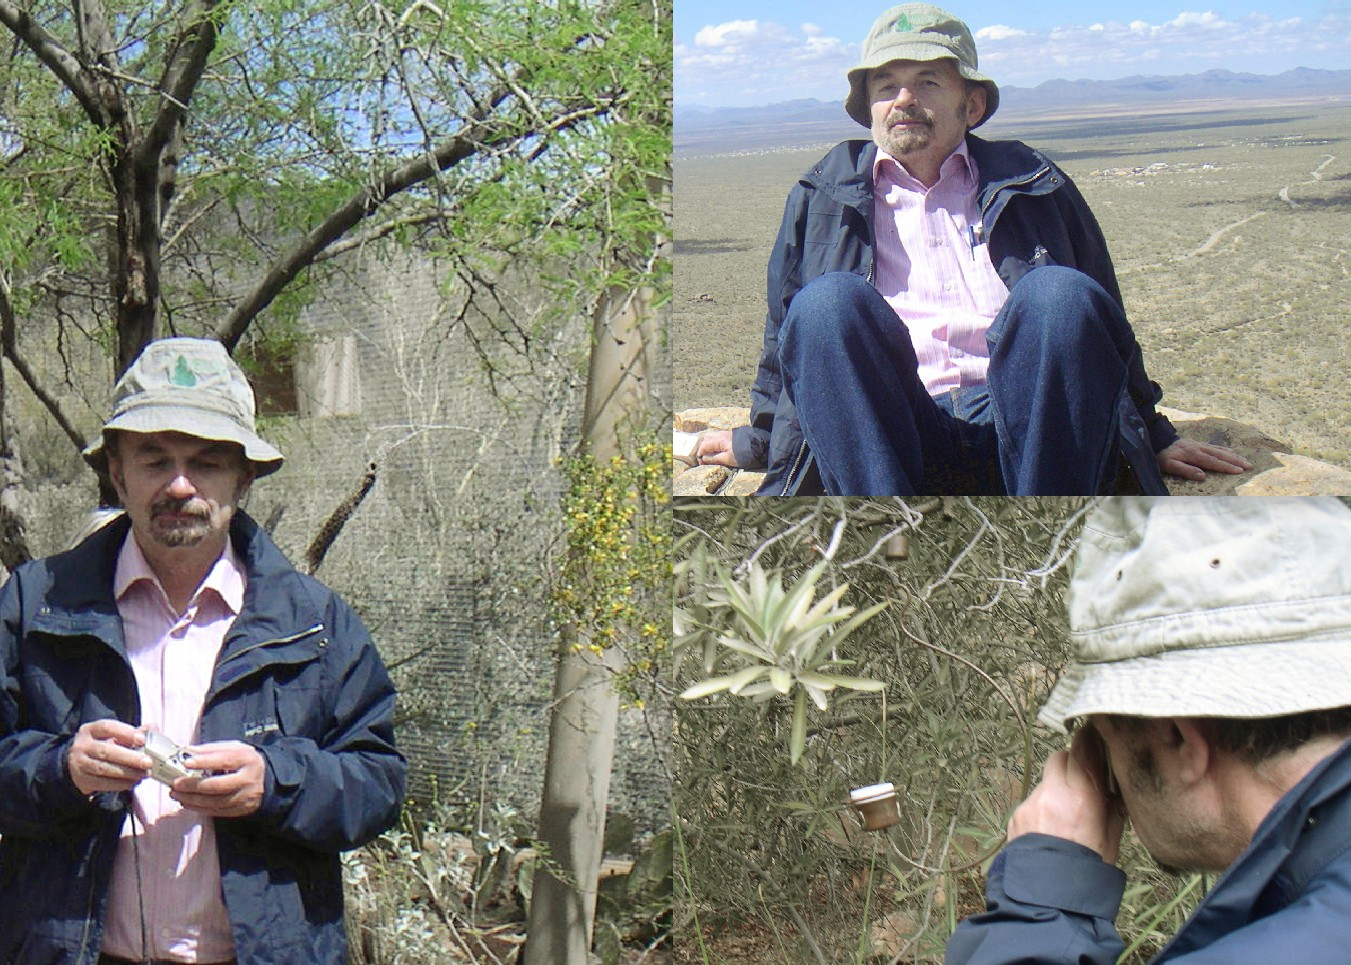
\includegraphics[width=0.95\columnwidth]{07March24HaraldCollageDesertMuseum.jpg}}
\caption{Harald Fritzsch visiting Arizona-Sonora Desert Museum in Spring 2007. Pictures and picture assembly by Johann Rafelski
}
\label{Fig:AZcolloq2007} 
\end{figure}

These meetings offered an opportunity to exchange ideas the  origin of neutrino mass and parameters of  the standard model were close to his heart. Were these parameters really natural constants on cosmological time scale? In Figure\,\ref{Fig:RANP2004} we see Harald's first transparency ``Time Dependence of QCD and Experimental Tests'' made at at the 9th Hadron Physics and 7th Relativistic Aspects of Nuclear Physics (HADRON-RANP 2004): A Joint Meeting on QCD and QGP: Rio de Janeiro, Brazil, March 28-April 3, 2004~\cite{Fritzsch:2004civ}, a meeting we both attended. We see that Harald modified slightly by hand the typed transparency to introduce the meeting specific context in a talk which arose from another publication of the epoch, Ref.\,\cite{Calmet:2001nu}. 

\begin{figure}%[ht]
\centerline{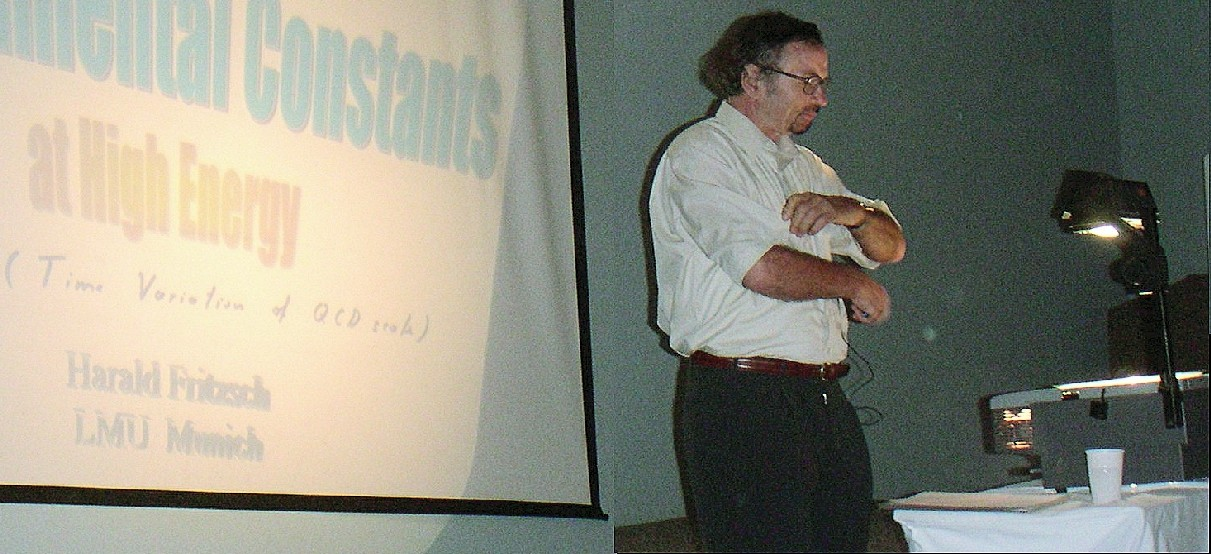
\includegraphics[width=0.95\columnwidth]{04RANPHarald1Ed.jpg}}
\caption{Harald begins his presentation in Rio de Janeiro 2004 about time dependence of QCD, see text for details. Picture by Johann Rafelski
}
\label{Fig:RANP2004} 
\end{figure}
 
%%%%%%%%%%%%%%%%%%%%%%%%%%%%%%%%%%%%


\bibliographystyle{ws-rv-van}
\bibliography{Rafelski_Steinmetz_for_Harald}
%%%%%%%%%%%%%%%%%%%%%%%%%%%%%%%%%%%%
\end{document} 
%%%%%%%%%%%%%%%%%%%%%%%%%%%%%%%%%%%%
